\documentclass[10pt]{article}
\usepackage[a4paper,margin=18mm]{geometry}
\usepackage[T1]{fontenc}\usepackage{lmodern}
\usepackage{amsmath,amssymb,booktabs,array,enumitem}
\usepackage{tikz}\usetikzlibrary{shapes.gates.logic.US,positioning,arrows.meta}
\usepackage[hidelinks]{hyperref}
\setlength{\parindent}{0pt}\setlength{\parskip}{4pt}\setlength{\emergencystretch}{2em}
\newcommand{\mos}[4]{\begin{scope}[shift={(#1,#2)}]
\draw(0,.24)--(0,-.24);\draw(0,.2)--(.25,.2)--(.25,.5);\draw(0,-.2)--(.25,-.2)--(.25,-.5);
\draw(-.16,.23)--(-.16,-.23);
\ifnum#4=1\draw(-.26,0)circle(.06);\draw(-.75,0)--(-.32,0);\else\draw(-.75,0)--(-.16,0);\fi
\node[anchor=east,font=\scriptsize]at(-.76,0){$#3$};\end{scope}}
\newcommand{\gnd}[2]{\draw(#1,#2)--(#1,{#2-.12});\draw({#1-.17},{#2-.12})--({#1+.17},{#2-.12});\draw({#1-.11},{#2-.2})--({#1+.11},{#2-.2});}
\newcommand{\rail}[3]{\draw(#1,#2)--(#1,{#2+.14});\node[above,font=\scriptsize]at(#1,{#2+.14}){$#3$};}
% ORIGINAL_LAYOUT_A / ORIGINAL_LAYOUT_B: normalized literal source topology.
% SOLUTION_LAYOUT_A / SOLUTION_LAYOUT_B: labelled MOS schematics, 12 devices each.
% Requires TikZ. No external image, style library, or custom circuit symbol needed.
\newcommand{\VLSIDiff}[2]{\fill[black!17] (#1,-.14) rectangle (#2,.14);\draw (#1,-.14) rectangle (#2,.14);}
\newcommand{\VLSIContact}[2]{\fill (#1-.075,#2-.075) rectangle (#1+.075,#2+.075);}
\newcommand{\VLSIRail}[3]{\draw[line width=3pt,black!35] (#1,#3)--(#2,#3);\draw (#1,#3-.085)--(#2,#3-.085) (#1,#3+.085)--(#2,#3+.085);}
\newcommand{\OriginalLayoutA}{%
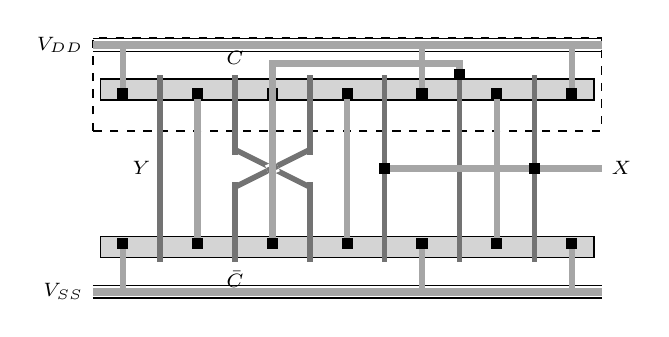
\begin{tikzpicture}[x=.95cm,y=.95cm,font=\scriptsize,line width=.5pt]
\draw[dashed] (-.4,.5) rectangle (6.4,1.75);
\begin{scope}[yshift=1cm]\VLSIDiff{-.3}{6.3}\end{scope}
\begin{scope}[yshift=-1cm]\VLSIDiff{-.3}{6.3}\end{scope}
\VLSIRail{-.4}{6.4}{1.65}\VLSIRail{-.4}{6.4}{-1.65}
\node[left] at (-.4,1.65) {$V_{DD}$};\node[left] at (-.4,-1.65) {$V_{SS}$};
% Six physical columns. Gate 1=Y; gate 2=C/Cbar; gate 3=Cbar/C;
% gate 4=X; gate 5=v; gate 6=X. Split clock gates are not shorted.
\foreach \x in {.5,3.5,4.5,5.5}{\draw[line width=2pt,black!55] (\x,-1.25)--(\x,1.25);}
\foreach \x in {1.5,2.5}{\draw[line width=2pt,black!55] (\x,.18)--(\x,1.25) (\x,-.18)--(\x,-1.25);}
\node[left] at (.5,0) {$Y$};\node[above] at (1.5,1.25) {$C$};\node[below] at (1.5,-1.25) {$\bar C$};
\draw[line width=2pt,black!55] (1.5,-.25)--(2.5,.25);\draw[line width=2pt,black!55] (1.5,.25)--(2.5,-.25);
% Opposite clock routes cross without a contact, shown with a bridge gap.
\draw[white,line width=4pt] (1.93,-.03)--(2.07,.03);\draw[line width=2pt,black!55] (1.93,-.03)--(2.07,.03);
% Supply contacts at physical channel intervals 0, 4, 6.
\foreach \x in {0,4,6}{\draw[line width=2.3pt,black!35] (\x,1)--(\x,1.65) (\x,-1)--(\x,-1.65);\VLSIContact{\x}{1}\VLSIContact{\x}{-1}}
% Inverter output u / transmission node v / feedback output r / X.
\foreach \x in {1,2,3,5}{\draw[line width=2.3pt,black!35] (\x,1)--(\x,-1);\VLSIContact{\x}{1}\VLSIContact{\x}{-1}}
\draw[line width=2.3pt,black!35] (2,.8)--(2,1.4)--(4.5,1.4)--(4.5,1.25);\VLSIContact{4.5}{1.25}
\draw[line width=2.3pt,black!35] (5,0)--(6.4,0) (3.5,0)--(5.5,0);\VLSIContact{3.5}{0}\VLSIContact{5.5}{0}
\node[right] at (6.4,0) {$X$};
\end{tikzpicture}}
\newcommand{\OriginalLayoutB}{%
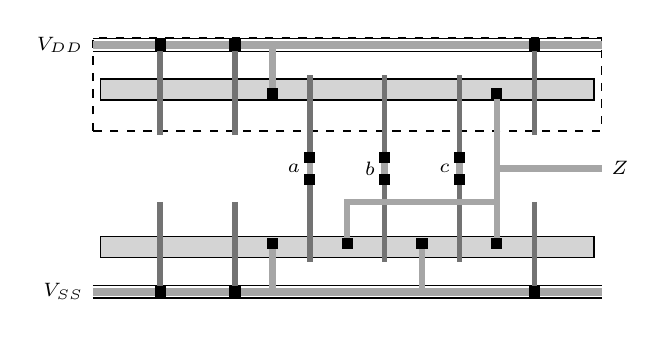
\begin{tikzpicture}[x=.95cm,y=.95cm,font=\scriptsize,line width=.5pt]
\draw[dashed] (-.4,.5) rectangle (6.4,1.75);
\begin{scope}[yshift=1cm]\VLSIDiff{-.3}{6.3}\end{scope}
\begin{scope}[yshift=-1cm]\VLSIDiff{-.3}{6.3}\end{scope}
\VLSIRail{-.4}{6.4}{1.65}\VLSIRail{-.4}{6.4}{-1.65}
\node[left] at (-.4,1.65) {$V_{DD}$};\node[left] at (-.4,-1.65) {$V_{SS}$};
\foreach \x in {.5,1.5,5.5}{\draw[line width=2pt,black!55] (\x,.45)--(\x,1.65) (\x,-.45)--(\x,-1.65);\VLSIContact{\x}{1.65}\VLSIContact{\x}{-1.65}}
\foreach \x/\g in {2.5/a,3.5/b,4.5/c}{\draw[line width=2pt,black!55] (\x,-1.25)--(\x,1.25);\draw[line width=2.3pt,black!35] (\x,-.15)--(\x,.15);\VLSIContact{\x}{-.15}\VLSIContact{\x}{.15}\node[left] at (\x,0) {$\g$};}
\draw[line width=2.3pt,black!35] (2,1)--(2,1.65) (2,-1)--(2,-1.65) (4,-1)--(4,-1.65);
\VLSIContact{2}{1}\VLSIContact{2}{-1}\VLSIContact{4}{-1}
\draw[line width=2.3pt,black!35] (5,1)--(5,-1) (3,-1)--(3,-.45)--(5,-.45);
\VLSIContact{5}{1}\VLSIContact{5}{-1}\VLSIContact{3}{-1}
\draw[line width=2.3pt,black!35] (5,0)--(6.4,0);\node[right] at (6.4,0) {$Z$};
\end{tikzpicture}}

\newcommand{\SolutionLayoutA}{%
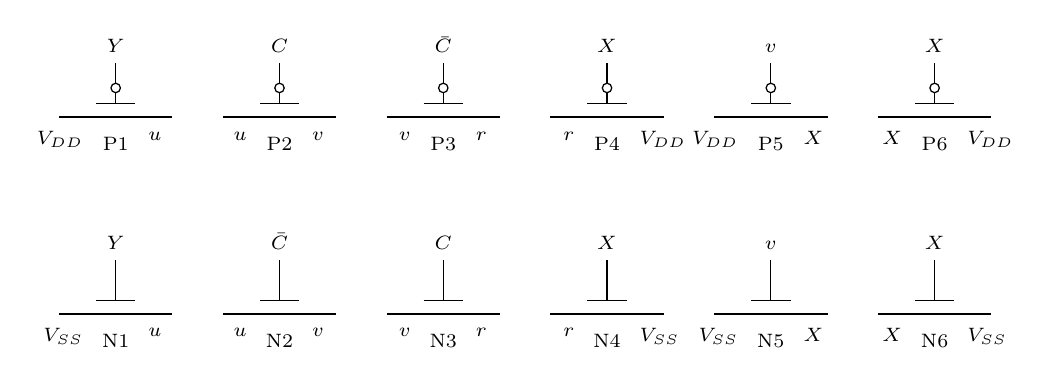
\begin{tikzpicture}[x=1cm,y=1cm,font=\scriptsize,line width=.45pt]
\draw (-0.72,2.5)--(-0.24,2.5) (0.24,2.5)--(0.72,2.5);
\draw[line width=1pt] (-0.24,2.5)--(0.24,2.5);
\draw (-0.25,2.67)--(0.25,2.67);
\draw (0.0,2.67)--(0.0,2.81);\draw (0.0,2.87) circle (.06);\draw (0.0,2.93)--(0.0,3.19);
\node[above] at (0.0,3.19) {$ Y $};
\node[below] at (0.0,2.37) {P1};
\node[anchor=north east] at (-0.29,2.44) {$ V_{DD} $};
\node[anchor=north west] at (0.29,2.44) {$ u $};
\draw (-0.72,0)--(-0.24,0) (0.24,0)--(0.72,0);
\draw[line width=1pt] (-0.24,0)--(0.24,0);
\draw (-0.25,0.17)--(0.25,0.17);
\draw (0.0,0.17)--(0.0,0.69);
\node[above] at (0.0,0.69) {$ Y $};
\node[below] at (0.0,-0.13) {N1};
\node[anchor=north east] at (-0.29,-0.06) {$ V_{SS} $};
\node[anchor=north west] at (0.29,-0.06) {$ u $};
\draw (1.36,2.5)--(1.84,2.5) (2.3200000000000003,2.5)--(2.8,2.5);
\draw[line width=1pt] (1.84,2.5)--(2.3200000000000003,2.5);
\draw (1.83,2.67)--(2.33,2.67);
\draw (2.08,2.67)--(2.08,2.81);\draw (2.08,2.87) circle (.06);\draw (2.08,2.93)--(2.08,3.19);
\node[above] at (2.08,3.19) {$ C $};
\node[below] at (2.08,2.37) {P2};
\node[anchor=north east] at (1.79,2.44) {$ u $};
\node[anchor=north west] at (2.37,2.44) {$ v $};
\draw (1.36,0)--(1.84,0) (2.3200000000000003,0)--(2.8,0);
\draw[line width=1pt] (1.84,0)--(2.3200000000000003,0);
\draw (1.83,0.17)--(2.33,0.17);
\draw (2.08,0.17)--(2.08,0.69);
\node[above] at (2.08,0.69) {$ \bar C $};
\node[below] at (2.08,-0.13) {N2};
\node[anchor=north east] at (1.79,-0.06) {$ u $};
\node[anchor=north west] at (2.37,-0.06) {$ v $};
\draw (3.4400000000000004,2.5)--(3.92,2.5) (4.4,2.5)--(4.88,2.5);
\draw[line width=1pt] (3.92,2.5)--(4.4,2.5);
\draw (3.91,2.67)--(4.41,2.67);
\draw (4.16,2.67)--(4.16,2.81);\draw (4.16,2.87) circle (.06);\draw (4.16,2.93)--(4.16,3.19);
\node[above] at (4.16,3.19) {$ \bar C $};
\node[below] at (4.16,2.37) {P3};
\node[anchor=north east] at (3.87,2.44) {$ v $};
\node[anchor=north west] at (4.45,2.44) {$ r $};
\draw (3.4400000000000004,0)--(3.92,0) (4.4,0)--(4.88,0);
\draw[line width=1pt] (3.92,0)--(4.4,0);
\draw (3.91,0.17)--(4.41,0.17);
\draw (4.16,0.17)--(4.16,0.69);
\node[above] at (4.16,0.69) {$ C $};
\node[below] at (4.16,-0.13) {N3};
\node[anchor=north east] at (3.87,-0.06) {$ v $};
\node[anchor=north west] at (4.45,-0.06) {$ r $};
\draw (5.5200000000000005,2.5)--(6.0,2.5) (6.48,2.5)--(6.96,2.5);
\draw[line width=1pt] (6.0,2.5)--(6.48,2.5);
\draw (5.99,2.67)--(6.49,2.67);
\draw (6.24,2.67)--(6.24,2.81);\draw (6.24,2.87) circle (.06);\draw (6.24,2.93)--(6.24,3.19);
\node[above] at (6.24,3.19) {$ X $};
\node[below] at (6.24,2.37) {P4};
\node[anchor=north east] at (5.95,2.44) {$ r $};
\node[anchor=north west] at (6.53,2.44) {$ V_{DD} $};
\draw (5.5200000000000005,0)--(6.0,0) (6.48,0)--(6.96,0);
\draw[line width=1pt] (6.0,0)--(6.48,0);
\draw (5.99,0.17)--(6.49,0.17);
\draw (6.24,0.17)--(6.24,0.69);
\node[above] at (6.24,0.69) {$ X $};
\node[below] at (6.24,-0.13) {N4};
\node[anchor=north east] at (5.95,-0.06) {$ r $};
\node[anchor=north west] at (6.53,-0.06) {$ V_{SS} $};
\draw (7.6000000000000005,2.5)--(8.08,2.5) (8.56,2.5)--(9.040000000000001,2.5);
\draw[line width=1pt] (8.08,2.5)--(8.56,2.5);
\draw (8.07,2.67)--(8.57,2.67);
\draw (8.32,2.67)--(8.32,2.81);\draw (8.32,2.87) circle (.06);\draw (8.32,2.93)--(8.32,3.19);
\node[above] at (8.32,3.19) {$ v $};
\node[below] at (8.32,2.37) {P5};
\node[anchor=north east] at (8.030000000000001,2.44) {$ V_{DD} $};
\node[anchor=north west] at (8.61,2.44) {$ X $};
\draw (7.6000000000000005,0)--(8.08,0) (8.56,0)--(9.040000000000001,0);
\draw[line width=1pt] (8.08,0)--(8.56,0);
\draw (8.07,0.17)--(8.57,0.17);
\draw (8.32,0.17)--(8.32,0.69);
\node[above] at (8.32,0.69) {$ v $};
\node[below] at (8.32,-0.13) {N5};
\node[anchor=north east] at (8.030000000000001,-0.06) {$ V_{SS} $};
\node[anchor=north west] at (8.61,-0.06) {$ X $};
\draw (9.68,2.5)--(10.16,2.5) (10.64,2.5)--(11.120000000000001,2.5);
\draw[line width=1pt] (10.16,2.5)--(10.64,2.5);
\draw (10.15,2.67)--(10.65,2.67);
\draw (10.4,2.67)--(10.4,2.81);\draw (10.4,2.87) circle (.06);\draw (10.4,2.93)--(10.4,3.19);
\node[above] at (10.4,3.19) {$ X $};
\node[below] at (10.4,2.37) {P6};
\node[anchor=north east] at (10.110000000000001,2.44) {$ X $};
\node[anchor=north west] at (10.69,2.44) {$ V_{DD} $};
\draw (9.68,0)--(10.16,0) (10.64,0)--(11.120000000000001,0);
\draw[line width=1pt] (10.16,0)--(10.64,0);
\draw (10.15,0.17)--(10.65,0.17);
\draw (10.4,0.17)--(10.4,0.69);
\node[above] at (10.4,0.69) {$ X $};
\node[below] at (10.4,-0.13) {N6};
\node[anchor=north east] at (10.110000000000001,-0.06) {$ X $};
\node[anchor=north west] at (10.69,-0.06) {$ V_{SS} $};
\end{tikzpicture}}
\newcommand{\SolutionLayoutB}{%
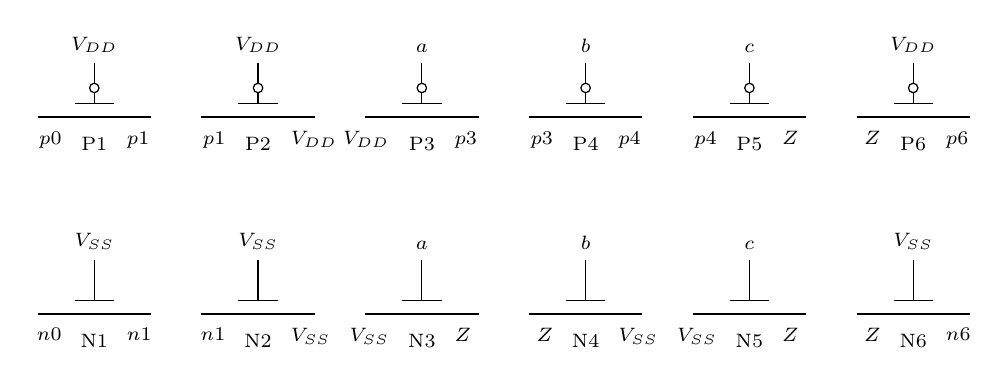
\begin{tikzpicture}[x=1cm,y=1cm,font=\scriptsize,line width=.45pt]
\draw (-0.72,2.5)--(-0.24,2.5) (0.24,2.5)--(0.72,2.5);
\draw[line width=1pt] (-0.24,2.5)--(0.24,2.5);
\draw (-0.25,2.67)--(0.25,2.67);
\draw (0.0,2.67)--(0.0,2.81);\draw (0.0,2.87) circle (.06);\draw (0.0,2.93)--(0.0,3.19);
\node[above] at (0.0,3.19) {$ V_{DD} $};
\node[below] at (0.0,2.37) {P1};
\node[anchor=north east] at (-0.29,2.44) {$ p0 $};
\node[anchor=north west] at (0.29,2.44) {$ p1 $};
\draw (-0.72,0)--(-0.24,0) (0.24,0)--(0.72,0);
\draw[line width=1pt] (-0.24,0)--(0.24,0);
\draw (-0.25,0.17)--(0.25,0.17);
\draw (0.0,0.17)--(0.0,0.69);
\node[above] at (0.0,0.69) {$ V_{SS} $};
\node[below] at (0.0,-0.13) {N1};
\node[anchor=north east] at (-0.29,-0.06) {$ n0 $};
\node[anchor=north west] at (0.29,-0.06) {$ n1 $};
\draw (1.36,2.5)--(1.84,2.5) (2.3200000000000003,2.5)--(2.8,2.5);
\draw[line width=1pt] (1.84,2.5)--(2.3200000000000003,2.5);
\draw (1.83,2.67)--(2.33,2.67);
\draw (2.08,2.67)--(2.08,2.81);\draw (2.08,2.87) circle (.06);\draw (2.08,2.93)--(2.08,3.19);
\node[above] at (2.08,3.19) {$ V_{DD} $};
\node[below] at (2.08,2.37) {P2};
\node[anchor=north east] at (1.79,2.44) {$ p1 $};
\node[anchor=north west] at (2.37,2.44) {$ V_{DD} $};
\draw (1.36,0)--(1.84,0) (2.3200000000000003,0)--(2.8,0);
\draw[line width=1pt] (1.84,0)--(2.3200000000000003,0);
\draw (1.83,0.17)--(2.33,0.17);
\draw (2.08,0.17)--(2.08,0.69);
\node[above] at (2.08,0.69) {$ V_{SS} $};
\node[below] at (2.08,-0.13) {N2};
\node[anchor=north east] at (1.79,-0.06) {$ n1 $};
\node[anchor=north west] at (2.37,-0.06) {$ V_{SS} $};
\draw (3.4400000000000004,2.5)--(3.92,2.5) (4.4,2.5)--(4.88,2.5);
\draw[line width=1pt] (3.92,2.5)--(4.4,2.5);
\draw (3.91,2.67)--(4.41,2.67);
\draw (4.16,2.67)--(4.16,2.81);\draw (4.16,2.87) circle (.06);\draw (4.16,2.93)--(4.16,3.19);
\node[above] at (4.16,3.19) {$ a $};
\node[below] at (4.16,2.37) {P3};
\node[anchor=north east] at (3.87,2.44) {$ V_{DD} $};
\node[anchor=north west] at (4.45,2.44) {$ p3 $};
\draw (3.4400000000000004,0)--(3.92,0) (4.4,0)--(4.88,0);
\draw[line width=1pt] (3.92,0)--(4.4,0);
\draw (3.91,0.17)--(4.41,0.17);
\draw (4.16,0.17)--(4.16,0.69);
\node[above] at (4.16,0.69) {$ a $};
\node[below] at (4.16,-0.13) {N3};
\node[anchor=north east] at (3.87,-0.06) {$ V_{SS} $};
\node[anchor=north west] at (4.45,-0.06) {$ Z $};
\draw (5.5200000000000005,2.5)--(6.0,2.5) (6.48,2.5)--(6.96,2.5);
\draw[line width=1pt] (6.0,2.5)--(6.48,2.5);
\draw (5.99,2.67)--(6.49,2.67);
\draw (6.24,2.67)--(6.24,2.81);\draw (6.24,2.87) circle (.06);\draw (6.24,2.93)--(6.24,3.19);
\node[above] at (6.24,3.19) {$ b $};
\node[below] at (6.24,2.37) {P4};
\node[anchor=north east] at (5.95,2.44) {$ p3 $};
\node[anchor=north west] at (6.53,2.44) {$ p4 $};
\draw (5.5200000000000005,0)--(6.0,0) (6.48,0)--(6.96,0);
\draw[line width=1pt] (6.0,0)--(6.48,0);
\draw (5.99,0.17)--(6.49,0.17);
\draw (6.24,0.17)--(6.24,0.69);
\node[above] at (6.24,0.69) {$ b $};
\node[below] at (6.24,-0.13) {N4};
\node[anchor=north east] at (5.95,-0.06) {$ Z $};
\node[anchor=north west] at (6.53,-0.06) {$ V_{SS} $};
\draw (7.6000000000000005,2.5)--(8.08,2.5) (8.56,2.5)--(9.040000000000001,2.5);
\draw[line width=1pt] (8.08,2.5)--(8.56,2.5);
\draw (8.07,2.67)--(8.57,2.67);
\draw (8.32,2.67)--(8.32,2.81);\draw (8.32,2.87) circle (.06);\draw (8.32,2.93)--(8.32,3.19);
\node[above] at (8.32,3.19) {$ c $};
\node[below] at (8.32,2.37) {P5};
\node[anchor=north east] at (8.030000000000001,2.44) {$ p4 $};
\node[anchor=north west] at (8.61,2.44) {$ Z $};
\draw (7.6000000000000005,0)--(8.08,0) (8.56,0)--(9.040000000000001,0);
\draw[line width=1pt] (8.08,0)--(8.56,0);
\draw (8.07,0.17)--(8.57,0.17);
\draw (8.32,0.17)--(8.32,0.69);
\node[above] at (8.32,0.69) {$ c $};
\node[below] at (8.32,-0.13) {N5};
\node[anchor=north east] at (8.030000000000001,-0.06) {$ V_{SS} $};
\node[anchor=north west] at (8.61,-0.06) {$ Z $};
\draw (9.68,2.5)--(10.16,2.5) (10.64,2.5)--(11.120000000000001,2.5);
\draw[line width=1pt] (10.16,2.5)--(10.64,2.5);
\draw (10.15,2.67)--(10.65,2.67);
\draw (10.4,2.67)--(10.4,2.81);\draw (10.4,2.87) circle (.06);\draw (10.4,2.93)--(10.4,3.19);
\node[above] at (10.4,3.19) {$ V_{DD} $};
\node[below] at (10.4,2.37) {P6};
\node[anchor=north east] at (10.110000000000001,2.44) {$ Z $};
\node[anchor=north west] at (10.69,2.44) {$ p6 $};
\draw (9.68,0)--(10.16,0) (10.64,0)--(11.120000000000001,0);
\draw[line width=1pt] (10.16,0)--(10.64,0);
\draw (10.15,0.17)--(10.65,0.17);
\draw (10.4,0.17)--(10.4,0.69);
\node[above] at (10.4,0.69) {$ V_{SS} $};
\node[below] at (10.4,-0.13) {N6};
\node[anchor=north east] at (10.110000000000001,-0.06) {$ Z $};
\node[anchor=north west] at (10.69,-0.06) {$ n6 $};
\end{tikzpicture}}
\begin{document}
\begin{center}{\Large 2012 Final: Corrected Independent Solutions}\end{center}
\textbf{Scope.} All original Q1--Q8, printed total 140 points, are available. The Fall 2012 footer establishes the year. The original photographs were read first, and both local handwritten answer sets A and B (four images each) were then compared. Marks and grades are provenance, not evidence that an answer is correct. Student identities are omitted. All diagrams here are editable TikZ; the scanned originals are retained separately.

\textbf{Models.} Use the source's ON-resistor, ideal-clock, fixed gate-delay and stated square-law threshold approximations where applicable. Width-proportional gate capacitances follow the source. NMOS bodies connect to GND, pMOS bodies to $V_{DD}$. No private process model is redistributed and no SPICE simulation is claimed. A source inconsistency is answered by a feasibility proof rather than silently changing its premise.

\section*{Question 1: Definitions, design and logic families}
\begin{enumerate}[label=(\alph*)]
\item \textbf{Physical design} transforms the logical netlist into legal geometry: placement of cell instances, routing, power distribution and physical verification. \textbf{Instantiate a cell} means creating a particular occurrence of a reusable cell master and connecting its pins. An \textbf{instance} is that particular occurrence with its own name, connections, location and orientation; it is distinct from the master definition.
\item Two cell-library layout requirements are: (1) a common row height with aligned power/ground rails that abut legally; (2) widths on the placement-site grid and legal boundary/pin access so neighboring cells can be placed and routed without design-rule violations. Fixed width is not required for every cell.
\item Reduce the shared package/power return inductance by using additional short parallel VDD/GND connections; reduce simultaneous $di/dt$ by controlled slew or staged/staggered output switching. The inductive component is $\Delta V\simeq L\,di/dt$. More supply connections and slower switching attack different factors in this expression.
\item An n-dynamic gate precharges its output high and may discharge during evaluation. Direct same-phase cascading is unsafe because the precharged high output can prematurely discharge the next stage. CMOS domino puts a static inverter after each n-dynamic stage, making its evaluation output rise monotonically. NP domino alternates n-dynamic stages (high precharge, falling evaluation) and p-dynamic stages (low reset, rising evaluation), with the corresponding clock controls. Alternating polarity permits the required monotonic input direction without a restoring inverter between every pair; proper phase and input stability are still necessary.
\item The parenthesis \emph{switching power of a complex gate} distinguishes output-load switching power and internal-node switching power:
\[P_{sw,out}=\alpha_o C_oV_{dd}^2f,\qquad P_{sw,int}=\sum_i\alpha_i C_iV_{dd}^2f.\]
These formulas assume full swing and count 0-to-1 charging events. Partial swings require the actual transferred charge. Short-circuit power is a separate dynamic mechanism, included explicitly in Q3, and is not the second capacitive switching component requested here; leakage is not switching power.
\item Balance arrivals at reconvergent inputs, and minimize unbalanced/reconvergent paths or use hazard-free logic where needed (for example, add a consensus term that removes a static hazard). These reduce unnecessary internal/output transitions. Adding capacitance alone may filter a pulse but increases charging energy, so it is not an unconditional low-power rule.
\item Two major problems are charge sharing with initially low internal nodes and unsafe direct cascading of plain same-phase dynamic gates. Leakage-induced loss of retained charge is another valid dynamic-logic problem.
\item Basic CMOS domino realizes noninverting functions at its buffered outputs, and requires inputs to remain stable or make only the allowed 0-to-1 transitions during n-evaluation. It also requires an output inverter on each n-dynamic stage; arbitrary feedback or an unbuffered falling domino input is unsafe.
\item In a \textbf{core-limited} design, the logic/core area determines the required die dimensions. In a \textbf{pad-limited} design, the number and pitch of IO pads determine the perimeter and hence die size, even if the core would fit in a smaller area.
\end{enumerate}
\textbf{Comparison.} Both sets contain useful definitions and bounce mitigation. Retain the library-abutment and input-arrival explanations. B's output/internal switching distinction in (e) is appropriate; A's switching/short-circuit split and leakage explanation do not answer that exact parenthetical wording. Qualify any claim that dynamic logic is simply ``low power,'' and do not treat capacitive pulse filtering as cost-free.

\newpage\section*{Question 2: Dynamic and fully differential implementations}
Absorption gives $A(B+C)+C=AB+AC+C=AB+C$. Let $h=AB+C$; then
\[\boxed{f=\bar h=\overline{AB+C},\qquad g=h,\qquad f=(\bar A+\bar B)\bar C.}\]
The dynamic pull-down uses C in parallel with an A--B series path, plus the precharge pMOS and evaluation footer. It has five MOS. During $\phi=0$, $f$ precharges high; during $\phi=1$, it discharges exactly when $h=1$. No output inverter is inserted, because that would produce $h$ rather than $f$.

In the fully differential gate, the $f$ pull-down implements $h=AB+C$ and the $g$ pull-down implements $f=(\bar A+\bar B)\bar C$. Cross-coupled pMOS loads connect $V_{DD}$ to $f$ with gate $g$, and to $g$ with gate $f$. One side discharges and turns on the opposite pMOS, which restores the complementary high output. The core has six nMOS plus two pMOS, or eight devices; if only A/B/C are supplied, three CMOS input inverters add six devices, giving fourteen total. Each complementary input inverter is a pMOS/nMOS pair with both gates at its original input, tied drains at its complement, and sources at the rails.
\begin{center}\begin{tikzpicture}[scale=.85,font=\small]
\mos{0}{3.7}{\phi}{1}\rail{.25}{4.2}{V_{DD}}\draw(.25,3.2)--(.25,2.8);\draw(-1.25,2.8)--(1.75,2.8)node[right]{$f$};
\mos{-1.5}{2}{C}{0}\mos{1}{2}{A}{0}\mos{1}{.6}{B}{0}\draw(-1.25,2.8)--(-1.25,2.5);\draw(1.25,2.8)--(1.25,2.5);\draw(1.25,1.5)--(1.25,1.1);\draw(-1.25,1.5)--(-1.25,-.1)--(1.25,-.1);\draw(1.25,.1)--(1.25,-.1);\draw(.25,-.1)--(.25,-.4);\mos{0}{-.9}{\phi}{0}\gnd{.25}{-1.4}
\end{tikzpicture}\hspace{1cm}\begin{tikzpicture}[scale=.85,font=\small]
\mos{0}{3.7}{g}{1}\mos{5}{3.7}{f}{1}\rail{.25}{4.2}{V_{DD}}\rail{5.25}{4.2}{V_{DD}}\draw(.25,3.2)--(.25,2.8);\draw(5.25,3.2)--(5.25,2.8);
\draw(-1.25,2.8)--(1.75,2.8);\node[right]at(1.75,2.8){$f$};\draw(4.25,2.8)--(6.25,2.8);\node[right]at(6.25,2.8){$g$};
\mos{-1.5}{2}{C}{0}\mos{1}{2}{A}{0}\mos{1}{.6}{B}{0}\draw(-1.25,2.8)--(-1.25,2.5);\draw(1.25,2.8)--(1.25,2.5);\draw(1.25,1.5)--(1.25,1.1);\draw(-1.25,1.5)--(-1.25,-.1)--(1.25,-.1);\draw(1.25,.1)--(1.25,-.1);\gnd{.25}{-.1}
\mos{4}{2}{\bar A}{0}\mos{6}{2}{\bar B}{0}\draw(4.25,2.8)--(4.25,2.5);\draw(6.25,2.8)--(6.25,2.5);\draw(4.25,1.5)--(4.25,1.3)--(6.25,1.3)--(6.25,1.5);\draw(5.25,1.3)--(5.25,1.1);\mos{5}{.6}{\bar C}{0}\gnd{5.25}{.1}
\end{tikzpicture}\\Left: dynamic implementation (5 MOS). Right: fully differential core (8 MOS); equal net names connect both pMOS feedback gates to the opposite outputs. Three CMOS input inverters generate $\bar A,\bar B,\bar C$ if complements are not supplied.\end{center}
\begin{center}\begin{tabular}{ccc|cc}\toprule A&B&C&$f$&$g$\\\midrule
0&0&0&1&0\\0&0&1&0&1\\0&1&0&1&0\\0&1&1&0&1\\1&0&0&1&0\\1&0&1&0&1\\1&1&0&0&1\\1&1&1&0&1\\\bottomrule\end{tabular}\end{center}
\textbf{Comparison.} The handwritten logic concepts can be retained after applying absorption. Explicitly supply complementary inputs and cross-coupled gate connections; do not count free input complements or change the required output polarity. The verifier checks both transistor conduction graphs on all eight input combinations.

\newpage\section*{Question 3: Four-stage inverter-chain power}
Let $\tau_0=C_g/(\beta V_{dd})$ denote the source's delay unit. Both input edges in the original waveform span \textbf{two unit delays}. Each stage is balanced because its pMOS width is twice its nMOS width. The receiving stage's short-circuit power uses its \emph{incoming} slew, which is the preceding driver's output slew.
\begin{center}\begin{tabular}{c|ccccc}\toprule
Stage&$\beta_i/\beta$&Input cap.&Output load&Input slew&Output slew\\\midrule
1&1&$3C_g$&$6C_g$&$2\tau_0$&$6\tau_0$\\
2&2&$6C_g$&$12C_g$&$6\tau_0$&$6\tau_0$\\
3&4&$12C_g$&$24C_g$&$6\tau_0$&$6\tau_0$\\
4&8&$24C_g$&$C_L$&$6\tau_0$&$C_L/(8\beta V_{dd})$\\\bottomrule
\end{tabular}\end{center}
The chain's four supplied output nodes charge the listed output loads. The external stimulus driver that charges the first inverter's $3C_g$ input is outside the requested four-inverter power sum. Therefore
\[\boxed{P_{sw}=fV_{dd}^2(42C_g+C_L).}\]
Use the \emph{printed} voltage factor $(V_{dd}-V_t)^3$, without replacing it by a different textbook form. The short-circuit sum is
\begin{align*}
P_{sc}&=k(V_{dd}-V_t)^3f\,[\beta(2\tau_0)+2\beta(6\tau_0)+4\beta(6\tau_0)+8\beta(6\tau_0)]\\
&=86k\beta\tau_0(V_{dd}-V_t)^3f
=\frac{86kC_g}{V_{dd}}(V_{dd}-V_t)^3f.
\end{align*}
\[\boxed{P_{dynamic}=fV_{dd}^2(42C_g+C_L)+\frac{86kC_gf}{V_{dd}}(V_{dd}-V_t)^3.}\]
The last $C_L$ affects switching power and final output slew, but not the incoming slew of stage 4 in the stipulated power model.
\begin{center}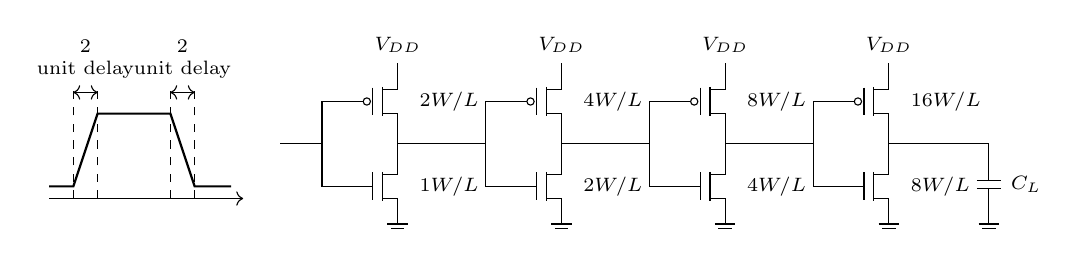
\begin{tikzpicture}[scale=.77,font=\scriptsize]
\begin{scope}[xshift=-5.5cm,yshift=.5cm]
\draw[->](0,0)--(3.2,0);\draw[thick](0,.2)--(.4,.2)--(.8,1.4)--(2,1.4)--(2.4,.2)--(3,.2);
\foreach \x in {.4,.8,2,2.4}{\draw[dashed](\x,0)--(\x,1.9);}
\draw[<->](.4,1.75)--(.8,1.75);\draw[<->](2,1.75)--(2.4,1.75);
\node[above,align=center]at(.6,1.82){2\\unit delay};\node[above,align=center]at(2.2,1.82){2\\unit delay};
\end{scope}
\foreach \x/\pn/\nn in {0/2/1,2.7/4/2,5.4/8/4,8.1/16/8}{
\mos{\x}{2.1}{}{1}\mos{\x}{.7}{}{0}\rail{\x+.25}{2.6}{V_{DD}}\gnd{\x+.25}{.2}
\draw(\x+.25,1.6)--(\x+.25,1.2);\draw(\x-.75,2.1)--(\x-1,2.1)--(\x-1,.7)--(\x-.75,.7);
\node[right]at(\x+.45,2.1){$\pn W/L$};\node[right]at(\x+.45,.7){$\nn W/L$};}
\draw(-1,1.4)--(-1.7,1.4);\draw(.25,1.4)--(1.7,1.4);\draw(2.95,1.4)--(4.4,1.4);\draw(5.65,1.4)--(7.1,1.4);\draw(8.35,1.4)--(10,1.4)--(10,.8);
\draw(9.8,.8)--(10.2,.8);\draw(9.8,.67)--(10.2,.67);\draw(10,.67)--(10,.2);\gnd{10}{.2}\node[right]at(10.2,.73){$C_L$};
\end{tikzpicture}\\Figure 1: An inverter chain driving a $C_L$.\end{center}
\textbf{Comparison.} Both sets correctly obtain the switching load sum. A applies each stage's own output slew in its short-circuit formula and incorrectly makes that power depend on $C_L$. B omits the increasing stage strength and arrives at an incorrect coefficient 11. Replace both short-circuit sums by the input-slew coefficients $2+12+24+48=86$. The printed ns unit is not an extra numerical factor to multiply twice.

\newpage\section*{Question 4: Sizing and proof of infeasibility}
Let $R_p$ be the ON resistance of the fixed $4\,\mu m$ P1. With all lengths $0.18\,\mu m$ and $\mu_n=2\mu_p$, an nMOS of width $W$ (in $\mu m$) has
\[\frac{R_n(W)}{R_p}=\frac{2}{W}.\]
The five individually sensitized discharge paths are X1--N1, X2--X3--N1, X2--X6--N1, X4--X5--X3--N1, and X4--X5--X6--N1. The shared middle junction of X2/X5/X3/X6 is retained in the analysis.

\textbf{(a)} One compact solution equalizes every individual path:
\begin{center}\begin{tabular}{c|rrrrrrr}\toprule
Device&X1&X2&X3&X4&X5&X6&N1\\\midrule
$W\ (\mu m)$&$8/3$&4&8&8&8&8&8\\
$R/R_p$&$3/4$&$1/2$&$1/4$&$1/4$&$1/4$&$1/4$&$1/4$\\\bottomrule
\end{tabular}\end{center}
Every listed path has resistance $R_p$ and therefore matches the precharge time for the same output capacitance. Additional parallel conducting paths are faster. This is a worst-case balance, not a claim that every multi-input state has the same fall time. All seven nMOS widths 8 $\mu m$ are also a valid simpler worst-case solution. Sizing is not unique: writing $r_i=R_i/R_p$, a family satisfies $r_3=r_6$, $r_2=r_4+r_5$, $r_1=r_2+r_3$, and $r_{N1}+r_3+r_4+r_5=1$, with all resistances positive.

\textbf{(b)} The clock drives only the fixed P1 gate ($C$) and footer N1 gate. Its switching power is
\[P_{CLK}=fCV_{dd}^2\left(1+\frac{W_{N1}}{4\,\mu m}\right).\]
The requested strict bound gives $W_{N1}<1\,\mu m$. But the footer alone is in every discharge path, and finite positive logic-device resistances require
\[R_{N1}<R_p\quad\Longrightarrow\quad W_{N1}>2\,\mu m\]
to match the rise time. Hence the original requirements are inconsistent:
\[\boxed{\text{No finite transistor sizing satisfies Q4(b).}}\]
In fact any finite balanced design requires $P_{CLK}>1.5fCV_{dd}^2$. The coefficient approaches 1.5 only as the footer approaches $2\,\mu m$ from above and logic widths tend to infinity; 1.5 is an infimum, not an achievable finite design. P1 was specified and is not a free variable.

\textbf{Comparison.} B's part (a) widths X1=4, X2=6, all remaining nMOS=8 $\mu m$ correctly match the worst path and may be retained. A's X3=6 makes the X4--X5--X3--N1 path $13R_p/12$ and fails balance. Both proposed part (b) footers violate the clock limit: the readable A footer 6 gives coefficient 2.5; B footer 8 gives 3. Neither is a solution. Exact conductance-matrix checks cover all 64 logic-control states for each of six compared designs.

\newpage\section*{Question 5: NP full-adder, correlated delays and sharing}
The original contains 22 devices: left n-dynamic stage 7, X p-clocked inverter 3, middle p-dynamic stage 9, Y n-clocked inverter 3. Call the original left dynamic node $z$, its internal nodes $x,y$, and the unlabelled middle dynamic output $w$. The controls A/B/C repeated in the middle gate are the same inputs, so their states cannot be independently chosen to construct a delay path.

In precharge ($\phi=0$), $z=1$, $X=0$, $w=0$, and $Y=1$. In evaluation ($\phi=1$), the left pull-down conducts for $M=AB+C(A+B)=AB+AC+BC$, so $z=\bar M$ and the p-clocked inverter gives $X=M$. The middle p network conducts for
\[(\bar A+\bar B+\bar C)(\bar z+\bar A\bar B\bar C).\]
After substituting $z=\bar M$, it gives even parity, $w=\overline{A\mathbin{\oplus}B\mathbin{\oplus}C}$; the last n-clocked inverter gives $Y=A\mathbin{\oplus}B\mathbin{\oplus}C$. Thus X is carry and Y is sum. Inputs must follow the required evaluation stability/monotonicity protocol; the result is not a static asynchronous truth table across arbitrary mid-cycle changes.

\textbf{(a) Loads and reachable delays.} Two pMOS gates load $z$, so $C_z=4C$. The last data nMOS gate loads $w$, so $C_w=C$. Neither X nor Y has an explicit external load and the source neglects drain capacitance, so the two terminal clocked-inverter stages contribute zero output RC in this ideal model. This is not a claim of zero physical output delay.

The z precharge is $t_{rz}=4RC$. With exactly two asserted inputs, its one conducting data path plus footer is $3R$: $t_{fz}=12RC$, $t_{dz}=8RC$. With ABC=111, the two data branches are $2R$ and $R+(R\parallel R)=3R/2$, whose parallel resistance is $6R/7$. Including the footer gives $13R/7$, hence
\[t_{fz}=\frac{52}{7}RC,\qquad t_{dz}=\frac12\left(4+\frac{52}{7}\right)RC=\frac{40}{7}RC.\]
For the middle stage, reset fall time is $RC$. ABC=000 has $z=1$, so the z-controlled pMOS is OFF: the header, three top pMOS in parallel, and three lower pMOS in series give $R+R/3+3R=13R/3$. Thus its mean delay is $8RC/3$. This is a primary-input-to-Y \emph{bypass} that does not require a z transition. With exactly two inputs high, only one top pMOS is ON, and falling z enables its parallel lower pMOS: header + top + z-pMOS gives $3R$ and mean delay $2RC$; the z-to-w-to-Y delay is $8RC+2RC=10RC$. With 111 the middle top network is OFF, so the fastest z transition does not yield a Y transition.
\begin{center}\begin{tabular}{c|ccccl}\toprule
ABC&$z$&X&$w$&Y&Reachable mean delays in $RC$\\\midrule
000&1&0&1&0&Y: $8/3$ (bypass)\\
001,010,100&1&0&0&1&No evaluation output transition\\
011,101,110&0&1&1&0&X: 8; Y: 10\\
111&0&1&0&1&X: $40/7$; no Y transition\\\bottomrule
\end{tabular}\end{center}
Following the question's \emph{per-gate average} $t_d=(t_r+t_f)/2$ convention and summing only reachable sensitized paths,
\[\boxed{X:\ [t_{cd},t_{pd}]=[40RC/7,8RC],\quad Y:\ [8RC/3,10RC],}\]
\[\boxed{\text{whole circuit: }t_{cd}=8RC/3,\qquad t_{pd}=10RC.}\]
These are the source-defined mean-delay metrics. Actual evaluation-only RC sums, if one instead followed only the active edge, would be $13RC/3$ for the bypass and $15RC$ for the longest z--w route; that is a different convention. Unspecified real output loads would add delay and are not silently invented.

\newpage\textbf{Q5(b): a valid charge-sharing counterexample.} Let z be precharged to 1.8 V while y initially retains 0 V. During evaluation choose ABC=001 (C asserts while A=B=0). The C device connects z to y; the A/B devices below y are OFF, and the A device leading to x is OFF. Therefore z shares with \emph{y only}, with no ground path:
\[V_{z,shared}=\frac{C_zV_{dd}+C_y(0)}{C_z+C_y}=\frac{1.6}{1.6+0.8}\,1.8=1.2\,V.\]
The z-controlled pMOS can turn on when $V_z<V_{dd}-|V_{tp}|=1.3\,V$. Since $1.2<1.3$, this valid floating-node history can falsely enable X and the middle p network. Thus correct operation is \textbf{not guaranteed} under the supplied ideal ON-sharing model. A low y state is reachable from an earlier evaluation; precharge does not independently charge y if C is OFF.

For comparison, ABC=100 connects z to x only, giving $1.6\cdot1.8/(1.6+0.4)=1.44\,V$, above the false-enable threshold. ABC=101 connects both x and y but also has a complete C--A--footer discharge path, so those three nodes cannot be pooled as an isolated charge-sharing capacitor set. Body effect, nMOS cutoff, leakage and analog transient waveforms are outside this simple model; no missing threshold value is fabricated.

\textbf{Comparison.} A omits the primary-input bypass and combines middle-gate device controls that cannot simultaneously occur, yielding an incorrect upper delay 11RC. Independently optimized stage bounds also cannot be added without checking shared-input reachability. Both students pool x+y+z and obtain approximately 1.03 V; that particular sharing scenario is invalid. Their qualitative malfunction concern is retained, with the valid z+y counterexample and 1.2 V calculation replacing it. All eight ABC states and all sixteen independent ABC/z states are saved for audit; the latter are explicitly flagged when inconsistent with the evaluated z function.

\newpage\section*{Question 6: Register-to-register timing}
Read the bubbles in the original: the lower gate is XNOR, the middle gate is XOR, and the last gate is XNOR. Defining registered outputs $q_i$,
\[D_3=\bar q_1,\quad D_4=q_3,\quad U=\overline{q_2+q_3},\quad D_5=U,\]
\[V=\overline{U\mathbin{\oplus}q_4},\quad W=V\mathbin{\oplus}q_5,\quad D_6=\overline{W\mathbin{\oplus}q_1}.\]
Combinational paths stop at a register, rather than passing through its D--Q boundary. The nine paths are
\begin{center}\begin{tabular}{llr}\toprule Launch&Capture and intervening logic&Delay (ns)\\\midrule
R1&R3: INV&0.3\\R1&R6: final XNOR&0.7\\R2&R5: NOR&0.7\\
R2&R6: NOR, lower XNOR, middle XOR, final XNOR&2.8\\
R3&R4: direct interconnection&$d_{34}$\\R3&R5: NOR&0.7\\
R3&R6: NOR, lower XNOR, middle XOR, final XNOR&2.8\\
R4&R6: lower XNOR, middle XOR, final XNOR&2.1\\R5&R6: middle XOR, final XNOR&1.4\\\bottomrule
\end{tabular}\end{center}
For pairwise skew $s_{ij}=t_{capture,j}-t_{launch,i}$, setup and hold require
\[T\ge t_{pcq}+d_{max,ij}+t_{setup}-s_{ij},\qquad t_{ccq}+d_{min,ij}\ge t_{hold}+s_{ij}.\]

\textbf{(a)} At zero skew the setup bound is $T\ge0.4+2.8+0.3=3.5\,ns$, giving a setup ceiling $f=285.714\,MHz$. However, the R3--R4 wire delay is not specified in (a). With the ordinary zero-wire idealization, $0.1+0<0.2$ violates hold; changing the clock period cannot fix it. Thus this is a \emph{setup-only ceiling} until the short path is repaired or an actual interconnect delay of at least 0.1 ns is established. Adding two 0.3 ns inverters on the R3--R4 branch restores its polarity and hold without changing the 2.8 ns critical path, making the ceiling attainable in the stated model.

\textbf{(b)} The unsigned ``0.5 ns skew'' has no launch/capture clock map. Conservatively interpreting it as a pairwise bound $|s_{ij}|\le0.5\,ns$, the adverse setup sign $s=-0.5$ requires $T\ge4.0\,ns$ and gives $\boxed{f\le250\,MHz}$. A favorable critical-pair sign $s=+0.5$ gives a setup-only ceiling $333.333\,MHz$, but makes hold stricter. Positive 0.5 ns pairwise skew requires each affected data path to have $d_{min}\ge0.2+0.5-0.1=0.6\,ns$. The 0.3 ns R1--R3 path and direct R3--R4 path need repair. Two additional inverters on each short branch give respectively 0.9 ns and 0.6 ns (or 0.65 ns with the wire in part c). Those branch repairs preserve function and the original critical delay. They make the conservative 250 MHz bound hold-safe. A uniform same-signed skew assigned independently to all pairs is not asserted to be a realizable single clock distribution.

\newpage\textbf{Q6(c): branch-only hold repair.} Now $d_{34}=0.05\,ns$ is explicitly given. At zero skew its hold arrival is $0.1+0.05=0.15\,ns<0.2\,ns$. Insert two existing 0.3 ns inverters on the \emph{R3-to-R4 branch only}, after the fanout to the NOR; the new data delay is $0.05+0.6=0.65\,ns$ and hold arrival is 0.75 ns. The branch's setup requirement is only $0.4+0.65+0.3=1.35\,ns<3.5\,ns$, so the 285.714 MHz ceiling is unchanged. Placing the buffer before the NOR fanout would unnecessarily slow the critical R3--R6 path.
\begin{center}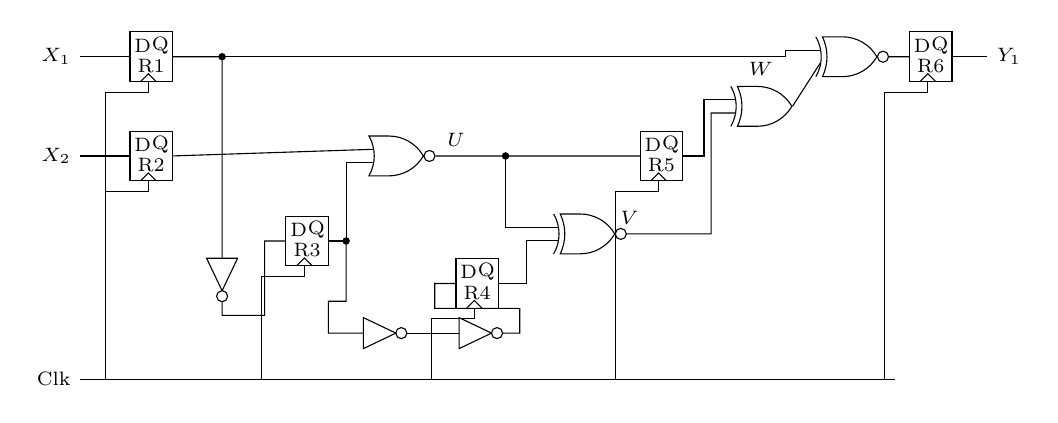
\begin{tikzpicture}[scale=.9,font=\scriptsize]
\draw(-0.3,2.85)rectangle(0.3,3.5500000000000003);\node at(-0.12,3.3600000000000003){D};\node at(0.13,3.3600000000000003){Q};\node at(0,3.0700000000000003){R1};
\draw(-0.15,2.85)--(-0.04,2.96)--(0.07,2.85);
\draw(-0.65,-1.35)--(-0.65,2.7)--(-0.04,2.7)--(-0.04,2.85);
\draw(-0.3,1.4500000000000002)rectangle(0.3,2.15);\node at(-0.12,1.96){D};\node at(0.13,1.96){Q};\node at(0,1.67){R2};
\draw(-0.15,1.4500000000000002)--(-0.04,1.56)--(0.07,1.4500000000000002);
\draw(-0.65,-1.35)--(-0.65,1.3)--(-0.04,1.3)--(-0.04,1.4500000000000002);
\draw(1.9000000000000001,0.25)rectangle(2.5,0.95);\node at(2.08,0.76){D};\node at(2.33,0.76){Q};\node at(2.2,0.47){R3};
\draw(2.0500000000000003,0.25)--(2.16,0.36)--(2.27,0.25);
\draw(1.5500000000000003,-1.35)--(1.5500000000000003,0.09999999999999998)--(2.16,0.09999999999999998)--(2.16,0.25);
\draw(4.3,-0.35)rectangle(4.8999999999999995,0.35);\node at(4.4799999999999995,0.16){D};\node at(4.7299999999999995,0.16){Q};\node at(4.6,-0.13){R4};
\draw(4.449999999999999,-0.35)--(4.56,-0.24)--(4.67,-0.35);
\draw(3.9499999999999997,-1.35)--(3.9499999999999997,-0.5)--(4.56,-0.5)--(4.56,-0.35);
\draw(6.9,1.4500000000000002)rectangle(7.5,2.15);\node at(7.08,1.96){D};\node at(7.33,1.96){Q};\node at(7.2,1.67){R5};
\draw(7.05,1.4500000000000002)--(7.16,1.56)--(7.2700000000000005,1.4500000000000002);
\draw(6.55,-1.35)--(6.55,1.3)--(7.16,1.3)--(7.16,1.4500000000000002);
\draw(10.7,2.85)rectangle(11.3,3.5500000000000003);\node at(10.88,3.3600000000000003){D};\node at(11.13,3.3600000000000003){Q};\node at(11,3.0700000000000003){R6};
\draw(10.85,2.85)--(10.96,2.96)--(11.07,2.85);
\draw(10.35,-1.35)--(10.35,2.7)--(10.96,2.7)--(10.96,2.85);
\draw(-1,-1.35)--(10.5,-1.35);\node[left]at(-1,-1.35){Clk};\draw(-.3,3.2)--(-1,3.2)node[left]{$X_1$};\draw(-.3,1.8)--(-1,1.8)node[left]{$X_2$};\draw(11.3,3.2)--(11.8,3.2)node[right]{$Y_1$};
\node[not gate US,draw,rotate=-90](i)at(1,.2){};\node[nor gate US,draw,logic gate inputs=nn](n)at(3.4,1.8){};
\node[xnor gate US,draw,logic gate inputs=nn](b)at(6.1,.7){};\node[xor gate US,draw,logic gate inputs=nn](m)at(8.6,2.5){};\node[xnor gate US,draw,logic gate inputs=nn](f)at(9.8,3.2){};
\draw(.3,3.2)--(1,3.2)--(i.input);\fill(1,3.2)circle(1.5pt);\draw(1,3.2)--(8.95,3.2)|-(f.input 1);
\draw(.3,1.8)--(n.input 1);\draw(2.5,.6)--(2.75,.6)|-(n.input 2);\fill(2.75,.6)circle(1.5pt);
\draw(n.output)--(5,1.8)--(6.9,1.8);\draw(5,1.8)|-(b.input 1);\fill(5,1.8)circle(1.5pt);\draw(4.9,0)--(5.3,0)|-(b.input 2);\draw(b.output)--(7.9,.7)|-(m.input 2);\draw(7.5,1.8)--(7.8,1.8)|-(m.input 1);\draw(m.output)--(f.input 2);\draw(f.output)--(10.7,3.2);
\node[above]at(4.3,1.8){$U$};\node[above]at(6.75,.7){$V$};\node[above]at(8.6,2.8){$W$};
\draw(i.output)--(1,-.45)--(1.6,-.45)--(1.6,.6)--(1.9,.6);
\node[not gate US,draw](d1)at(3.15,-.7){};\node[not gate US,draw](d2)at(4.5,-.7){};\draw(2.75,.6)--(2.75,-.25)--(2.5,-.25)--(2.5,-.7)--(d1.input);\draw(d1.output)--(d2.input);\draw(d2.output)--(5.2,-.7)--(5.2,-.35)--(4,-.35)--(4,0)--(4.3,0);
\end{tikzpicture}\\Figure 4, branch-only hold repair; existing fanout paths stay connected.\end{center}
\textbf{Comparison.} A's 3.5 ns setup bound, adverse-sign 250 MHz and two-inverter hold repair are useful; retain them with the explicit hold and skew qualifications. A's middle gate should be XOR. B incorrectly takes reciprocals of the hold-side minimum time to report GHz frequencies; hold does not determine a maximum frequency and its proposed zero-skew validity fails the short branch. The saved path checks independently enumerate all nine routes and all three pairwise skew envelopes.

\newpage\section*{Question 7: Literal extraction of both 12-MOS layouts}
Each source layout has six gate-crossing columns in each diffusion row: six pMOS in n-well and six nMOS, twelve total. Black contact squares join layers; mere crossings without a contact do not. The opposite clock routes in (a) remain distinct. Source/drain sides below identify the left/right physical channel intervals; MOS channels are treated bidirectionally in this symbolic extraction. Bodies are $V_{DD}$ for pMOS and $V_{SS}$ for nMOS.

\textbf{(a)} Introduce analysis-only nets $u,v,r$ to name the original connected intervals. The complete circuit is input inverter Y-to-u, complementary-clock transmission gates u--v and v--r, inverter with input X/output r, inverter with input v/output X, and the last self-connected pair at X. No last-column device is dropped or rewired.
\begin{center}\resizebox{\linewidth}{!}{\SolutionLayoutA}\end{center}
\begin{center}\begin{tabular}{c|ccc|ccc}\toprule
Column&pMOS left&pMOS right&p gate&nMOS left&nMOS right&n gate\\\midrule
1&$V_{DD}$&u&Y&$V_{SS}$&u&Y\\
2&u&v&C&u&v&$\bar C$\\
3&v&r&$\bar C$&v&r&C\\
4&r&$V_{DD}$&X&r&$V_{SS}$&X\\
5&$V_{DD}$&X&v&$V_{SS}$&X&v\\
6&X&$V_{DD}$&X&X&$V_{SS}$&X\\\bottomrule
\end{tabular}\end{center}
For C=0, u--v is ON and v--r is OFF; for C=1, u--v is OFF and v--r is ON. But the physical last p/n pair has gates at X and channels from X to the rails. At X=0 its pMOS pulls upward; at X=1 its nMOS pulls downward. It loads/clamps X and opposes rail-valued retention. This is the literal transistor-level answer requested; it cannot be described as a clean unmodified latch or silently repaired without changing the source. Actual analog levels/writeability depend on omitted device strengths.

\newpage\textbf{Q7(b): NOR core plus six physical OFF devices.}
The middle three pMOS are in series and the corresponding three nMOS in parallel, so the functional core is $Z=\overline{a+b+c}$. Columns 1, 2 and 6 have p gates tied to $V_{DD}$ and n gates to $V_{SS}$; these six devices are OFF in ordinary rail logic and leave floating stubs. They still appear in a complete physical schematic.
\begin{center}\resizebox{\linewidth}{!}{\SolutionLayoutB}\end{center}
\begin{center}\begin{tabular}{c|ccc|ccc}\toprule
Column&p left&p right&p gate&n left&n right&n gate\\\midrule
1&$p_0$&$p_1$&$V_{DD}$&$n_0$&$n_1$&$V_{SS}$\\
2&$p_1$&$V_{DD}$&$V_{DD}$&$n_1$&$V_{SS}$&$V_{SS}$\\
3&$V_{DD}$&$p_3$&a&$V_{SS}$&Z&a\\
4&$p_3$&$p_4$&b&Z&$V_{SS}$&b\\
5&$p_4$&Z&c&$V_{SS}$&Z&c\\
6&Z&$p_6$&$V_{DD}$&Z&$n_6$&$V_{SS}$\\\bottomrule
\end{tabular}\end{center}
Repeated named terminals in the diagrams are electrically connected, and distinct stub names denote distinct floating segments. The two CSV netlists retain all 24 devices. Verifiers check the NOR's supply conduction on all eight abc states and explicitly identify the self-connected final X pair in (a).

\textbf{Comparison.} A's incomplete (a) sketch cannot replace the original extraction. B's conventional latch interpretation omits or changes the final X pair. Both sets' NOR interpretation in (b) is useful for the functional core, but their schematic omits the six rail-gated OFF devices. Retain the correct NOR result and restore every physical transistor in the requested literal schematic.

\newpage\section*{Question 8: Schmitt upper-trip ratio from MOS currents}
The original explicitly specifies $V_{T+}=1.2\,V$, rather than merely drawing an input-noise peak. At the rising-input transition, assume the output remains high at $V_{dd}$ immediately before regeneration, and let $v_a$ be the internal node between N1 and N2. N2 starts conducting at $V_{in}-v_a=V_{tn}$, giving
\[v_a=V_{T+}-V_{tn}=1.2-0.6=0.6\,V.\]
For N1, $V_{GS}=1.2$, $V_{DS}=0.6$, and $V_{GS}-V_{tn}=0.6$ V: it is at the saturation boundary. For feedback N3, the source is $v_a=0.6$ V, gate and drain are at $V_{dd}=1.8$ V, so $V_{GS}=V_{DS}=1.2$ V and its overdrive is also 0.6 V; it is saturated. Balancing their currents in the fixed-threshold square-law approximation,
\[\tfrac12\beta_{N1}(V_{T+}-V_{tn})^2=\tfrac12\beta_{N3}(V_{dd}-V_{T+})^2,\]
\[\boxed{\frac{\beta_{N1}}{\beta_{N3}}=\left(\frac{V_{dd}-V_{T+}}{V_{T+}-V_{tn}}\right)^2=1.}\]
This onset model neglects body effect and channel-length modulation, consistent with the fixed threshold provided. It does not claim a complete analog VTC simulation or invent the pMOS threshold/lower trip.
\begin{center}\begin{tikzpicture}[scale=.91,font=\small]
\mos{0}{3.8}{}{1}\mos{0}{2.4}{}{1}\mos{0}{1}{}{0}\mos{0}{-.4}{}{0}
\rail{.25}{4.3}{V_{dd}}\draw(.25,3.3)--(.25,2.9);\draw(.25,1.9)--(.25,1.5);\draw(.25,.5)--(.25,.1);\gnd{.25}{-.9}
\draw(-.75,3.8)--(-1.25,3.8)--(-1.25,-.4)--(-.75,-.4);\draw(-1.25,2.4)--(-.75,2.4);\draw(-1.25,1)--(-.75,1);\draw(-1.25,1.7)--(-1.8,1.7)node[left]{$V_{in}$};
\node[right]at(.4,3.8){P1};\node[right]at(.4,2.4){P2};\node[right]at(.4,1){N2};\node[right]at(.4,-.4){N1};
\draw(.25,3.1)--(1.15,3.1);\begin{scope}[shift={(1.65,2.85)},rotate=90]\mos{0}{0}{}{1}\end{scope}\draw(2.15,3.1)--(2.5,3.1);\gnd{2.5}{3.1}\node[above]at(1.6,3.28){P3};
\draw(.25,.3)--(1.15,.3);\begin{scope}[shift={(1.65,.55)},rotate=-90]\mos{0}{0}{}{0}\end{scope}\draw(2.15,.3)--(2.5,.3);\rail{2.5}{.3}{V_{dd}}\node[below]at(1.6,-.2){N3};
\draw(.25,1.7)--(3.3,1.7)node[right]{$V_{out}$};\fill(.25,1.7)circle(1.5pt);\draw(1.65,2.1)--(1.65,1.3);\fill(1.65,1.7)circle(1.5pt);
\begin{scope}[xshift=5.5cm]
\draw[->](0,0)--(4.4,0)node[right]{$V_{in}$};\draw[->](0,0)--(0,3.7)node[above]{$V_{out}$};\node[left]at(0,3){$V_{dd}$};
\draw[thick](0,3)--(2.2,3)..controls(2.75,3)and(2.9,2.4)..(2.9,1.4)..controls(2.9,.3)and(3.4,0)..(4,0);
\draw[thick](0,3)--(.5,3)..controls(1.2,3)and(1.4,2.5)..(1.4,1.4)..controls(1.4,.3)and(2.1,0)..(4,0);
\draw[dashed](1.4,0)--(1.4,1.4);\draw[dashed](2.9,0)--(2.9,1.4);\draw[->](1.85,3)--(2.2,3);\draw[->](2.9,2)--(2.9,1.5);\draw[->](1.4,1.5)--(1.4,2);\draw[->](2.2,0)--(1.85,0);
\node[below]at(1.4,0){$V_{T-}$};\node[below]at(2.9,0){$V_{T+}$};\node[below]at(4,0){$V_{dd}$};\node at(1.8,-.9){(b)};\end{scope}\node at(.7,-1.55){(a)};
\end{tikzpicture}\\Figure 6: (a) A CMOS Schmitt circuit. (b) Its voltage transfer curve.\end{center}
\textbf{Comparison.} Both student sets use a constant-resistance divider and infer ratio 2. That substitution is incorrect for these different drain biases. Even with equal $\beta$, both carry the same onset current but N3 has $V_{DS}=1.2$ V while N1 has 0.6 V, so their \emph{effective} $V_{DS}/I_D$ resistances differ by two. That effective resistance difference does not imply a beta ratio of two. The required beta ratio is one under the stated MOS-current approximation.

\section*{Reproducible verification}
Run \texttt{python verify.py}. Its standard-library checks regenerate the saved CSV/JSON evidence: Q2 conduction on all eight inputs; Q3 stage loads/slews; Q4 all 64 control patterns for six compared sizing schemes and the analytical clock-power contradiction; Q5 all eight reachable ABC states, all sixteen independent ABC/z states with consistency flags, and sharing components; Q6 all nine register paths under zero/adverse/favorable pairwise skew envelopes and branch repairs; Q7 complete literal netlists and NOR truth; Q8 onset currents and operating regions. These are analytical checks, not transistor simulations. The reconstructed circuit diagrams remain editable and retain the printed connections. Student comparisons are anonymized in \texttt{student-comparison.csv}.
\end{document}